\subsection{Pseudocódigo relevante a los métodos de interpolación}
\par \IEEEPARstart{A}{} continuaci\'on nos explayaremos sobre los detalles de la
implementaci\'on del m\'etodo propuesto. En las secciones previas hemos dado una
introducci\'on al problema, su modelo y justificaci\'on de por qué el mismo sirve
y a su vez hemos expuesto un m\'etodo que nos permite hayar la soluci\'on.

$f(x) = a + b (x - x0)$

$y0 + (y1-y0) * ( (x - x0) / (x1 - x0)) \implies a = y0 \ y \ b = (y1-y0)/(x1-x0)$

\begin{algorithm}
    \KwIn{Puntos del dominio conocidos $x$ ; Puntos de im\'agen conocidos $y$, grado funci\'on $gr$}
    \KwOut{Vector coeficiente $a$, Vector coeficiente $b$}
    
    \For{$i = 1 \ldots gr-1$}
    {		
		$a_i \gets y_i$\;
		$b_i \gets \frac{y_{i+1} - y_{i} }{x_{i+1} - x_{i}}$\;
	}
    \KwRet{$a$,$b$}
    \caption{Pseudoc\'odigo del algoritmo de Interpolaci\'on lineal}
    \label{alg:int_lineal}
\end{algorithm}

$f(x) = d + c ( x - x0 ) + b ( x - x0)^2 + a ( x - x0)^3$

\begin{algorithm}
    \KwIn{Puntos del dominio conocidos $x$ ; Puntos de im\'agen conocidos $y$, grado funci\'on $gr$}
    \KwOut{Vector coeficiente $a$, Vector coeficiente $b$, Vector coeficinete $c$, Vector coeficiente $d$}
    
	$MatrizSplines(0,0) \gets  1$\;
	$MatrizSplines(1,0) \gets  0$\;
	$vectorIndep_0 \gets 0$\;    
    
    \For{$i = 2 \ldots gr-1$}
    {		
		$MatrizSplines(i,i-1) \gets x_i - x_{i-1}$\;
		$MatrizSplines(i,i) \gets 2 \ (x_{i+1} - x_{i-1})$\;
		$MatrizSplines(i,i+1) \gets (x_{i+1} - x_i)$\;
		$vectorIndep_i \gets 3 \  \frac{y_{i+1} - y_i }{x_{i+1}- x_{i}} - \frac{y_i - y_{i-1}}{ x_i -x_{i-1}}$\;
	}    
	
	$MatrizSplines(gr,gr) \gets  1$\;
	$MatrizSplines(gr,gr-1) \gets  0$\;
	$vectorIndep_{gr} \gets 0$\; 
	
	$b \gets ResolverSistemaEcuaciones(MatrizSplines,vectorIndep)$\;
	
	\For{$i = 1 \ldots gr$}
	{
		$a_i \gets \frac{1}{3 \ \frac{b_{i+1} - b_{i}}{x_{i+1} - x_i}}$\;
		$b_i \gets \frac{y_{i+1}- y_i}{x_{i+1}- x_i} - \frac{1}{3 \ (2 \ b_i + b_{i+1}) * (x_{i+1} - x_{i})}$\;
	}    
	
	$y \gets d$	
	
    \KwRet{$a$,$b$,$c$,$d$}
    \caption{Pseudoc\'odigo del algoritmo de Interpolaci\'on por Splines}
    \label{alg:int_splines}
\end{algorithm}


El algoritmo de vecino mas cercano es simplemente copiar los frames apropiadamente como se explicó en la sección Desarrollo.

\subsection{Diseño del programa}
Desde un punto de vista de diseño, se explicarán brevemente las decisiones tomadas acerca de estructuras de datos y flujo de datos desde el video de input hasta el video de output. Se mencionarán además, posibles mejoras que quedaron fuera de este trabajo por cuestiones de tiempo.\\

\emph{Nota:} Se ignorarán partes del programa hechas específicamente para la experimentacion, centrándonos únicamente en el efecto de slowmotion sobre un video de entrada.\\

Se tienen los siguientes renombres y estructuras:
\begin{itemize}
	\item Pixel: Byte sin signo.
	\item Frame: Conjunto ordenado en 2 dimensiones de píxeles.
	\item Video: Metadata del video\footnote{Ancho, Alto, Fps, Cantidad de frames.} y un conjunto ordenado de frames.
\end{itemize}

Representamos los conjuntos ordenados como arreglos, utilizando el contenedor \emph{vector} de la libreria STL de C++.\\

Explicaremos en órden de procesamiento las etapas del flujo de datos:
\begin{enumerate}
	\item Lectura del video de disco a Ram: Se utilizó la librería \emph{OpenCV} para leer un video desde un stream y guardarlo en una estructura Video mencionada anteriormente. Se lee el video completo a RAM, convirtiendolo a blanco y negro mediante una función provista por la librería.
	\item Se procesa el video según el método de interpolación elegido y sus parámetros asociados. En caso de interpolación lineal o vecino más cercano, simplemente se itera entre todos los pares de frames consecutivos generando segun corresponda los frames intermedios. En el caso de splines, se divide el video en bloques de un tamaño determinado y se calcula un spline para cada pixel dentro de cada bloque\footnote{Los bloques consecutivos comparten el mismo último y primer pixel para evitar saltos en la interpolación.}\footnote{Se arma el sistema de ecuaciones de splines y se resuelve mediante eliminación gaussiana.}. Luego, se procede a generar frames intermedios evaluando estos splines para cada pixel, en el punto intermedio correspondiente.\\
	\emph{Nota:} El procesamiento de un video de entrada se traduce en la creación de un video de salida donde sus frames son una sucesión de frames originales y frames generados intercalados.
	\item Finalmente, se realiza el proceso opuesto con \emph{OpenCV}, se escribe desde una estructura Video, a una stream binario con un formato de video determinado. La conversión de color de escala de grises a RGB es directamente replicar la intensidad de brillo en cada componente de color.
\end{enumerate}

\begin{figure}[h!]
  \begin{centering}
    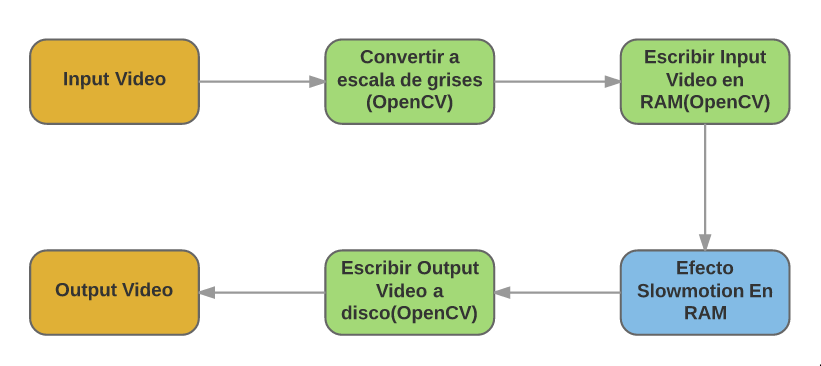
\includegraphics[width=0.55\textwidth]{img/dataflow.png}
     \caption{Flujo de procesamiento de datos del video}\label{fig:dataflow}
 \end{centering}
\end{figure}

Como posibles mejoras se tienen:
\begin{itemize}
	 \item Leer el video de forma \emph{lazy} y escribir de forma \emph{golosa}, es decir, leer de disco a ram únicamente el conjunto de frames necesarios para trabajar\footnote{El tamaño de bloque spline en interpolación spline, o 2 píxeles en los otros métodos.}, generar nuevos frames e ir escribiendolos al resultado a medida que se generan. Esto minimizaría el uso de la memoría RAM, respecto a la solución actual que mantiene todo el video de input y output en RAM antes de escribir a disco. 

	 \item Aprovechar la forma tridiagonal de la matriz del sistema lineal que queda al resolver un spline utilizando una matriz esparsa, y/o alguna factorización apropiada. 
\end{itemize}



